\section{Consuntivo di periodo} \label{section:consuntivo}
Questa sezione riporta le spese effettivamente sostenute dal gruppo \groupName.
Vengono riportate le ore ed i costi impiegati in ciascun ruolo per svolgere le attività pianificate.
Viene inoltre presentato un bilancio in termini di costo, dato dalla differenza tra il consuntivo di periodo ed il preventivo, che potrà essere:
\begin{itemize}
  \item \textbf{Positivo:} Se la spesa effettiva è minore di quanto preventivato;
  \item \textbf{In pareggio:} Se la spesa effettiva è uguale a quanto preventivato;
  \item \textbf{Negativo:} Se la spesa effettiva è maggiore di quanto preventivato.
\end{itemize}
Il bilancio viene riportato tra parentesi a fianco dei valori rilevati dal consuntivo di periodo.
\\Se il valore tra parentesi non è presente indica che l'aspettativa del preventivo è stata rispettata.

%%%%%%%%%%%%%%%%%%%%%%%%%%%%%%%%%%%%%%%%%%%%%%%%%%%%%%%%%%%%%%

\subsection{Analisi preliminare} \label{subsection:consuntivo_analisi}
\subsubsection{Variazione della pianificazione} \label{subsubsection:variazione_pianificazione_analisi}
\begin{table}[H]
  \centering
  \renewcommand{\arraystretch}{1.8}
  \rowcolors{2}{green!100!black!40}{green!100!black!30}
  \begin{tabular}{c|c|c|c|c|c|c|c}
    \rowcolor[HTML]{125E28}
    \multicolumn{1}{c}{\color[HTML]{FFFFFF}\textbf{ Nominativo }}
                         & \multicolumn{1}{c}{\color[HTML]{FFFFFF}\textbf{ Re }}
                         & \multicolumn{1}{c}{\color[HTML]{FFFFFF}\textbf{ Am}}
                         & \multicolumn{1}{c}{\color[HTML]{FFFFFF}\textbf{ An }}
                         & \multicolumn{1}{c}{\color[HTML]{FFFFFF}\textbf{ Pt }}
                         & \multicolumn{1}{c}{\color[HTML]{FFFFFF}\textbf{ Pr }}
                         & \multicolumn{1}{c}{\color[HTML]{FFFFFF}\textbf{ Ve }}
                         & \multicolumn{1}{c}{\color[HTML]{FFFFFF}\textbf{ Ore totali }}                                                                                    \\
    \hline
    Bugno Francesco      & 11 (+2)                                                       & -           & 9           & -          & -          & 11 (-2)     & 31           \\
    Busacca Luca         & -                                                             & 17          & 5           & -          & -          & 9  (-1)     & 31 (-1)      \\
    Carturan Luca        & 12 (+1)                                                       & 5 (+1)      & 5           & -          & -          & 9  (-2)     & 31           \\
    Filosofo Michele     & -                                                             & 5 (+2)      & 15 (-2)     & -          & -          & 11          & 31           \\
    Furlan Dario         & -                                                             & -           & 19 (-1)     & -          & -          & 12          & 31 (-1)      \\
    Mattarello Francesco & -                                                             & 15          & 6           & -          & -          & 10 (-1)     & 31 (-1)      \\
    Midena Matteo        & -                                                             & -           & 23 (-1)     & -          & -          & 9           & 32 (-1)      \\
    \textbf{Ore totali}  & \textbf{26}                                                   & \textbf{45} & \textbf{79} & \textbf{-} & \textbf{-} & \textbf{65} & \textbf{214}
  \end{tabular}
  \caption{Variazione delle ore nel periodo di Analisi preliminare}
\end{table}

\subsubsection{Variazione dei costi} \label{subsubsection:variazione_costi_analisi}
\begin{table}[H]
  \centering
  \renewcommand{\arraystretch}{1.8}
  \rowcolors{2}{green!100!black!40}{green!100!black!30}
  \begin{tabular}{c|c|c}
    \rowcolor[HTML]{125E28}
    \multicolumn{1}{c}{\color[HTML]{FFFFFF}\textbf{Ruolo}}
                               & \multicolumn{1}{c}{\color[HTML]{FFFFFF}\textbf{Ore}}
                               & \multicolumn{1}{c}{\color[HTML]{FFFFFF}\textbf{Costo (€)}}                     \\
    \hline
    Responsabile               & 26 (+3)                                                    & 780,00 (+90,00)   \\
    Amministratore             & 45 (+3)                                                    & 900,00 (+60,00)   \\
    Analista                   & 78 (-4)                                                    & 1950,00 (-100,00) \\
    Progettista                & -                                                          & -                 \\
    Programmatore              & -                                                          & -                 \\
    Verificatore               & 65 (-6)                                                    & 975,00 (-90,00)   \\
    \textbf{Totale Consuntivo} & \textbf{214}                                               & \textbf{4605,00}  \\
    \textbf{Totale Preventivo} & \textbf{218}                                               & \textbf{4645,00}  \\
    \textbf{Bilancio}          & \textbf{-4}                                                & \textbf{-40,00}   \\
  \end{tabular}
  \caption{Analisi preliminare - Consuntivo di periodo}
\end{table}


\subsubsection{Ragione degli scostamenti} \label{subsubsection:ragione_scostamenti_analisi}
\begin{itemize}
  \item \textbf{Responsabile (+3 ore):} Inizialmente, a causa dell'inesperienza, tale figura ha riscontrato problemi nella suddivisione del carico del lavoro, richiedendo un'analisi più minuziosa;
  \item \textbf{Amministratore (+3 ore):} La stesura delle \docNameNdP\ ha richiesto più tempo del previsto data l'elevata dipendenza con gli altri documenti;
  \item \textbf{Analista (-4 ore):} Grazie alle conoscenze pregresse di alcuni membri del gruppo si è riusciti ad ottimizzare i tempi previsti per l'\docNameAdR;
  \item \textbf{Verificatore (-6 ore):} Durante questo periodo, avendo solamente documentazione da verificare, il controllo è risultato più rapido del previsto.
\end{itemize}

\subsubsection{Considerazioni rispetto al preventivo} \label{subsubsection:considerazioni_finali_analisi}
Il bilancio risulta essere positivo rispetto al preventivo per questo periodo. Non si ritiene comunque necessaria alcuna ripianificazione del prossimo periodo in quanto la somma risparmiata non è abbastanza significativa.
Inoltre, avendo raggiunto tutti gli obiettivi precedentemente pianificati, l'avanzamento delle attività non ha subito alcun rallentamento.
\pagebreak
%%%%%%%%%%%%%%%%%%%%%%%%%%%%%%%%%%%%%%%%%%%%%%%%%%%%%%%%%%%%%%

\subsection{Progettazione Technology Baseline} \label{subsection:consuntivo_TB}
\subsubsection{Variazione della pianificazione} \label{subsubsection:variazione_pianificazione_TB}

\begin{table}[H]
  \centering
  \renewcommand{\arraystretch}{1.8}
  \rowcolors{2}{green!100!black!40}{green!100!black!30}
  \begin{tabular}{c|c|c|c|c|c|c|c}
    \rowcolor[HTML]{125E28}
    \multicolumn{1}{c}{\color[HTML]{FFFFFF}\textbf{ Nominativo }}
                         & \multicolumn{1}{c}{\color[HTML]{FFFFFF}\textbf{ Re }}
                         & \multicolumn{1}{c}{\color[HTML]{FFFFFF}\textbf{ Am}}
                         & \multicolumn{1}{c}{\color[HTML]{FFFFFF}\textbf{ An }}
                         & \multicolumn{1}{c}{\color[HTML]{FFFFFF}\textbf{ Pt }}
                         & \multicolumn{1}{c}{\color[HTML]{FFFFFF}\textbf{ Pr }}
                         & \multicolumn{1}{c}{\color[HTML]{FFFFFF}\textbf{ Ve }}
                         & \multicolumn{1}{c}{\color[HTML]{FFFFFF}\textbf{ Ore totali }}                                                                                   \\
    \hline
    Bugno Francesco      & -                                                             & 2          & 3           & 3 (-1)      & -          & 3 (-1)      & 11 (-2)     \\
    Busacca Luca         & -                                                             & -          & -           & 6 (-1)      & -          & 4 (-1)      & 10 (-2)     \\
    Carturan Luca        & -                                                             & -          & 5 (-1)      & 6 (-1)      & -          & -           & 11 (-2)     \\
    Filosofo Michele     & -                                                             & 3          & -           & 4 (-1)      & -          & 4 (-1)      & 11 (-2)     \\
    Furlan Dario         & 7 (-2)                                                        & -          & -           & 5           & -          & -           & 12 (-2)     \\
    Mattarello Francesco & -                                                             & -          & 4           & 4 (-1)      & -          & 3 (-1)      & 11 (-2)     \\
    Midena Matteo        & -                                                             & 3 (-1)     & -           & 5 (-1)      & -          & 3           & 11 (-2)     \\
    \textbf{Ore totali}  & \textbf{5}                                                    & \textbf{7} & \textbf{11} & \textbf{27} & \textbf{-} & \textbf{13} & \textbf{63}
  \end{tabular}
  \caption{Variazione delle ore nel periodo di Progettazione Technology Baseline}
\end{table}

\subsubsection{Variazione dei costi} \label{subsubsection:variazione_costi_TB}

\begin{table}[H]
  \centering
  \renewcommand{\arraystretch}{1.8}
  \rowcolors{2}{green!100!black!40}{green!100!black!30}
  \begin{tabular}{c|c|c}
    \rowcolor[HTML]{125E28}
    \multicolumn{1}{c}{\color[HTML]{FFFFFF}\textbf{Ruolo}} &
    \multicolumn{1}{c}{\color[HTML]{FFFFFF}\textbf{Ore}}   &
    \multicolumn{1}{c}{\color[HTML]{FFFFFF}\textbf{Costo (€)}}                               \\
    \hline
    Responsabile                                           & 5 (-2)       & 150,00 (-60,00)  \\
    Amministratore                                         & 7 (-1)       & 140,00 (-20,00)  \\
    Analista                                               & 11 (-1)      & 275,00 (-25,00)  \\
    Progettista                                            & 27 (-6)      & 675,00 (-150,00) \\
    Programmatore                                          & -            & -                \\
    Verificatore                                           & 13 (-4)      & 195,00 (-60,00)  \\
    \textbf{Totale Consuntivo}                             & \textbf{63}  & \textbf{1435,00} \\
    \textbf{Totale Preventivo}                             & \textbf{77}  & \textbf{1750,00} \\
    \textbf{Bilancio}                                      & \textbf{-14} & \textbf{-315,00} \\
  \end{tabular}
  \caption{Progettazione Technology Baseline - Consuntivo di periodo}
\end{table}


\subsubsection{Ragione degli scostamenti} \label{subsubsection:ragione_scostamenti_TB}
A causa dell'inizio della sessione d'esame si è deciso di apportare una variazione della pianificazione inizialmente preventivata per dare la possibilità ai singoli membri del gruppo di potersi dedicare allo studio individuale.
Di comune accordo si è pensato di ridurre per ciascun membro le ore totali da dedicare al progetto in modo equilibrato e sensato per non stravolgere il normale flusso di lavoro.

\subsubsection{Considerazioni rispetto al preventivo} \label{subsubsection:considerazioni_finali_TB}
Il bilancio risulta essere positivo rispetto al preventivo per questo periodo.
A causa del minor tempo che il gruppo è riuscito a dedicare al progetto in questo periodo si è ritenuto necessaria una ripianificazione del perido successivo.
Non avendo raggiunto tutti gli obiettivi precedentemente pianificati il gruppo ha deciso di attribuire maggiore importanza al ruolo di \roleDesignerLow\ e \roleProgrammerLow, incrementandone le ore di lavoro, per riuscire a rispettare il più possibile la pianificazione iniziale e non sforare con le tempistiche.

\paragraph{Codifica Proof of Concept - Preventivo a finire} \label{paragraph:preventivo_finire_Poc}

\subparagraph{Prospetto orario} \label{subparagraph:prospetto_orario_PoC}
\begin{table}[H]
  \centering
  \renewcommand{\arraystretch}{1.8}
  \rowcolors{2}{green!100!black!40}{green!100!black!30}
  \begin{tabular}{c|c|c|c|c|c|c|c}
    \rowcolor[HTML]{125E28}
    \multicolumn{1}{c}{\color[HTML]{FFFFFF}\textbf{ Nominativo }}
                         & \multicolumn{1}{c}{\color[HTML]{FFFFFF}\textbf{ Re }}
                         & \multicolumn{1}{c}{\color[HTML]{FFFFFF}\textbf{ Am}}
                         & \multicolumn{1}{c}{\color[HTML]{FFFFFF}\textbf{ An }}
                         & \multicolumn{1}{c}{\color[HTML]{FFFFFF}\textbf{ Pt }}
                         & \multicolumn{1}{c}{\color[HTML]{FFFFFF}\textbf{ Pr }}
                         & \multicolumn{1}{c}{\color[HTML]{FFFFFF}\textbf{ Ve }}
                         & \multicolumn{1}{c}{\color[HTML]{FFFFFF}\textbf{ Ore totali }}                                                                                    \\
    \hline
    Bugno Francesco      & -                                                             & -          & -          & 7 (+1)      & 4 (+2)      & 6           & 17 (+3)      \\
    Busacca Luca         & -                                                             & -          & 3          & 5 (+2)      & 7           & 4           & 19 (+2)      \\
    Carturan Luca        & -                                                             & -          & -          & 6 (+1)      & 8 (+2)      & 3           & 17 (+3)      \\
    Filosofo Michele     & -                                                             & -          & 4          & 4 (+2)      & 7           & 3           & 18 (+2)      \\
    Furlan Dario         & -                                                             & 2          & -          & 8 (+1)      & 8 (+1)      & -           & 18 (+2)      \\
    Mattarello Francesco & -                                                             & 3 (-1)     & -          & 6 (+1)      & 2 (+2)      & 7           & 18 (+2)      \\
    Midena Matteo        & 8 (-2)                                                        & -          & -          & 2 (+3)      & 8 (+1)      & -           & 18 (+2)      \\
    \textbf{Ore totali}  & \textbf{6}                                                    & \textbf{4} & \textbf{7} & \textbf{49} & \textbf{52} & \textbf{23} & \textbf{141}
  \end{tabular}
  \caption{Distribuzione delle ore nel periodo di Codifica Proof of Concept\glo - Preventivo a finire}
\end{table}

I valori sono riassunti graficamente nel seguente grafico:
\begin{figure}[H]
  \centering
  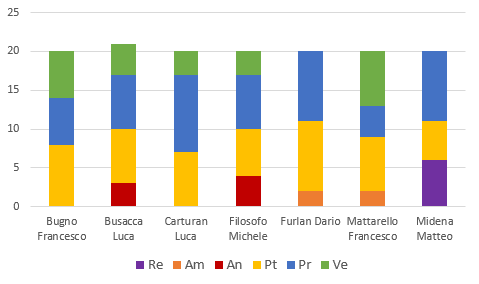
\includegraphics[scale=0.9]{immagini/ore_lavoro_preventivo_finire_PoC.png}
  \caption{Distribuzione ore di lavoro periodo di Codifica Proof of Concept\glo - Preventivo a finire}
\end{figure}

\subparagraph{Prospetto economico} \label{subparagraph:prospetto_economico_PoC}

\begin{table}[H]
  \centering
  \renewcommand{\arraystretch}{1.8}
  \rowcolors{2}{green!100!black!40}{green!100!black!30}
  \begin{tabular}{c|c|c}
    \rowcolor[HTML]{125E28}
    \multicolumn{1}{c}{\color[HTML]{FFFFFF}\textbf{Ruolo}}
                    & \multicolumn{1}{c}{\color[HTML]{FFFFFF}\textbf{Ore}}
                    & \multicolumn{1}{c}{\color[HTML]{FFFFFF}\textbf{Costo (€)}}                              \\
    \hline
    Responsabile    & 6 (-2)                                                     & 180,00 (-60,00)            \\
    Amministratore  & 4 (-1)                                                     & 80,00 (-20,00)             \\
    Analista        & 7                                                          & 175,00                     \\
    Progettista     & 49 (+11)                                                   & 1225,00 (+275,00)          \\
    Programmatore   & 52 (+8)                                                    & 780,00 (+120,00)           \\
    Verificatore    & 23                                                         & 345,00                     \\
    \textbf{Totale} & \textbf{141 (+16)}                                         & \textbf{2785,00 (+315,00)} \\
  \end{tabular}
  \caption{Prospetto delle ore e dei costi per ruolo nel periodo di Codifica Proof of Concept\glo - Preventivo a finire}
\end{table}

\begin{figure}[H]
  \centering
  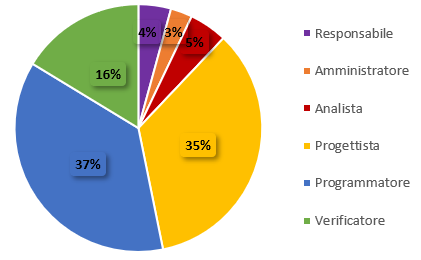
\includegraphics[scale=0.9]{immagini/ore_ruolo_preventivo_finire_PoC.png}
  \caption{Suddivisione delle ore di lavoro per ruolo sul totale per il periodo di Codifica Proof of Concept- Preventivo a finire}
\end{figure}


%%%%%%%%%%%%%%%%%%%%%%%%%%%%%%%%%%%%%%%%%%%%%%%%%%%%%%%%%%%%%%

\paragraph{Progettazione di dettaglio e codifica requisiti obbligatori - Preventivo a finire} \label{paragraph:preventivo_finire_reqObbligatori}
Per ora la pianificazione di questo periodo rimane invariata rispetto a quella iniziale.
Successivamente alla revisione \RTB \ , se necessario, verrà aggiornata la pianificazione riguardante questo periodo.
\paragraph{Progettazione di dettaglio e codifica requisiti opzionali - Preventivo a finire} \label{paragraph:preventivo_finire_reqOpzionali}
Per ora la pianificazione di questo periodo rimane invariata rispetto a quella iniziale.
Successivamente alla revisione \RTB \ , se necessario, verrà aggiornata la pianificazione riguardante questo periodo.
\paragraph{Validazione e collaudo - Preventivo a finire} \label{paragraph:preventivo_finire_Validazione}
Per ora la pianificazione di questo periodo rimane invariata rispetto a quella iniziale.
Successivamente alla revisione \RTB \ , se necessario, verrà aggiornata la pianificazione riguardante questo periodo.

\subsubsection{Conclusioni} \label{subsubsection:conclusioni}
Il totale delle ore rendicontate preventivate per il progetto diventa il seguente:

\begin{table}[H]
  \centering
  \renewcommand{\arraystretch}{1.8}
  \rowcolors{2}{green!100!black!40}{green!100!black!30}
  \begin{tabular}{c|c|c|c|c|c|c|c}
    \rowcolor[HTML]{125E28}
    \multicolumn{1}{c}{\color[HTML]{FFFFFF}\textbf{ Nominativo }}
                         & \multicolumn{1}{c}{\color[HTML]{FFFFFF}\textbf{ Re }}
                         & \multicolumn{1}{c}{\color[HTML]{FFFFFF}\textbf{ Am}}
                         & \multicolumn{1}{c}{\color[HTML]{FFFFFF}\textbf{ An }}
                         & \multicolumn{1}{c}{\color[HTML]{FFFFFF}\textbf{ Pt }}
                         & \multicolumn{1}{c}{\color[HTML]{FFFFFF}\textbf{ Pr }}
                         & \multicolumn{1}{c}{\color[HTML]{FFFFFF}\textbf{ Ve }}
                         & \multicolumn{1}{c}{\color[HTML]{FFFFFF}\textbf{ Ore totali }}                                                                                          \\
    \hline
    Bugno Francesco      & 11 (+2)                                                       & 5           & 12           & 20           & 23 (+2)      & 29 (-3)      & 100 (+1)     \\
    Busacca Luca         & 4                                                             & 17          & 10           & 20 (+1)      & 25           & 24 (-2)      & 100 (-1)     \\
    Carturan Luca        & 12 (+1)                                                       & 5 (+1)      & 10 (-1)      & 23           & 28 (+2)      & 22 (-2)      & 100 (+1)     \\
    Filosofo Michele     & 6                                                             & 8 (+2)      & 19 (-2)      & 24 (+1)      & 17           & 26 (-1)      & 100          \\
    Furlan Dario         & 7 (-2)                                                        & 10          & 19 (-1)      & 24 (+1)      & 15 (+1)      & 25           & 100 (-1)     \\
    Mattarello Francesco & 7                                                             & 18 (-1)     & 12           & 23           & 16 (+2)      & 24 (-2)      & 100 (-1)     \\
    Midena Matteo        & 8 (-2)                                                        & 7 (-1)      & 23 (-1)      & 16 (+2)      & 26 (+1)      & 20           & 100 (-1)     \\
    \textbf{Ore totali}  & \textbf{54}                                                   & \textbf{71} & \textbf{100} & \textbf{155} & \textbf{158} & \textbf{160} & \textbf{698}
  \end{tabular}
  \caption{Riepilogo della distribuzione oraria totale rendicontata - Preventivo a finire}
\end{table}

\begin{figure}[H]
  \centering
  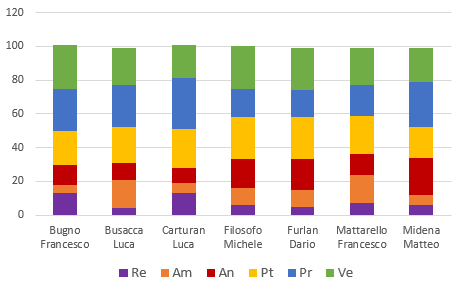
\includegraphics[scale=0.9]{immagini/ore_lavoro_preventivo_finire.png}
  \caption{Istogramma della distribuzione oraria totale rendicontata - Preventivo a finire}
\end{figure}


\begin{table}[H]
  \centering
  \renewcommand{\arraystretch}{1.8}
  \rowcolors{2}{green!100!black!40}{green!100!black!30}
  \begin{tabular}{c|c|c}
    \rowcolor[HTML]{125E28}
    \multicolumn{1}{c}{\color[HTML]{FFFFFF}\textbf{Ruolo}}
                    & \multicolumn{1}{c}{\color[HTML]{FFFFFF}\textbf{Ore}}
                    & \multicolumn{1}{c}{\color[HTML]{FFFFFF}\textbf{Costo (€)}}                              \\
    \hline
    Responsabile    & 54 (-1)                                                    & 1620,00 (-30,00)           \\
    Amministratore  & 71 (+1)                                                    & 1420,00 (+20,00)           \\
    Analista        & 100 (-5)                                                   & 2500,00 (-125,00)          \\
    Progettista     & 155 (+5)                                                   & 3875,00 (+125,00)          \\
    Programmatore   & 158 (+8)                                                   & 2370,00 (+120,00)          \\
    Verificatore    & 160 (-10)                                                  & 2400,00 (-150,00)          \\
    \textbf{Totale} & \textbf{698 (-2)}                                          & \textbf{14185,00 (-40,00)} \\
  \end{tabular}
  \caption{Prospetto delle ore e dei costi delle ore rendicontate - Preventivo a finire}
\end{table}

\begin{figure}[H]
  \centering
  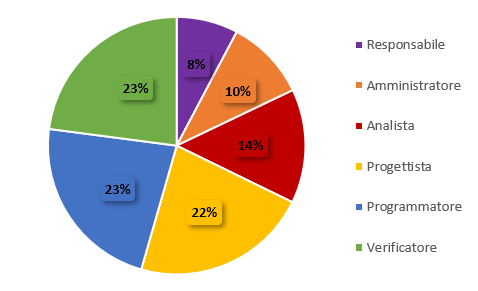
\includegraphics[scale=0.9]{immagini/ore_ruolo_preventivo_finire.png}
  \caption{Aerogramma delle ore per ruolo rendicontate sul totale- Preventivo a finire}
\end{figure}

Il carico di ore a persona è leggermente diminuito e il preventivo a finire scende a 14185,00€.

\pagebreak
%%%%%%%%%%%%%%%%%%%%%%%%%%%%%%%%%%%%%%%%%%%%%%%%%%%%%%%%%%%%%%

\subsection{Preventivo a finire} \label{subsection:preventivo_a_finire}
Di seguito viene riportato il preventivo a finire mediante una tabella.
Per ogni periodo che è stato ultimato viene riportato il preventivo ed il consuntivo di periodo.
Se il valore del consuntivo di un periodo non risulta essere ancora presente, per il conteggio del totale verrà utilizzato il valore del preventivo.
\begin{table}[H]
  \centering
  \renewcommand{\arraystretch}{1.8}
  \rowcolors{2}{green!100!black!40}{green!100!black!30}
  \begin{tabular}{c|c|c}
    \rowcolor[HTML]{125E28}
    \multicolumn{1}{c}{\color[HTML]{FFFFFF}\textbf{Periodo}}
                                      & \multicolumn{1}{c}{\color[HTML]{FFFFFF}\textbf{Preventivo}}
                                      & \multicolumn{1}{c}{\color[HTML]{FFFFFF}\textbf{Consuntivo}}                     \\
    \hline
    Analisi preliminare               & 4645,00                                                     & 4605,00           \\
    Progettazione Technology Baseline & 1750,00                                                     & 1435,00           \\
    Codifica Proof of Concept         & 2470,00                                                     & -                 \\
    \textbf{Totale}                   & \textbf{14225,00}                                           & \textbf{13870,00} \\
  \end{tabular}
  \caption{Preventivo a finire}
\end{table}


